%%%%%%%%%%%%%%%%%%%%%%%%%%%%%%%%%%%%%%%%%%%%%%%%%%%%%%%%%%%%%%%%%%%%%%%%%%%%%%%%%%%%%%%%%%
\section{Evaluation}
\label{s:eval}
%%%%%%%%%%%%%%%%%%%%%%%%%%%%%%%%%%%%%%%%%%%%%%%%%%%%%%%%%%%%%%%%%%%%%%%%%%%%%%%%%%%%%%%%%%i

%
Our performance evaluation focuses on the Lobsters, WebSubmit, and HotCRP applications
from our case studies.
%
We seek to answer the four questions:
%
\begin{enumerate}[nosep]
 %
 \item Does \sys meet its security goals and provide meaningful guarantees to users?
   (\S\ref{s:eval-security})
 %
 \item How expensive are core \sys interactions, \emph{viz.}\ disguising, revealing, and
   operations over disguised data? (\S\ref{s:eval-ops})
 %
 \item How much does application latency and storage use increase when an application
   uses \sys? (\S\ref{s:eval-res})
 %
 \item How do disguise and reveal actions impact the performance of concurrently executing,
   normal application requests by other users? (\S\ref{s:eval-conc})
 %
\end{enumerate}
%
All benchmarks run on a 40-core server with Intel Xeon E5-2660 v3 CPUs and 64 GB RAM,
running Arch Linux 5.15.7.
%
We use the MariaDB RDMS with the InnoDB storage engine for application data storage, but
store all databases on \fn{tmpfs} to avoid confounding factors related to persistence.
%

\subsection{Security Evaluation}
\label{s:eval-security}

%
An attacker who compromises the server observes all application
database content, the public metadata in \sys, and the (encrypted) contents of
\sys's store.
%
The attacker can learn:
\begin{enumerate}[nosep]
  \item the disguise specifications, from application code;
  \item any undisguised data in the application database;
  \item the number of encrypted bags in \sys and their sizes;
  \item the active natural principals, via \sys's list of
    registered principal public keys and the application DB;
  \item the IDs of all pseudoprincipals in existence, from \sys's metadata
    and the application DB;
  \item the IDs of deleted pseudoprincipals who still have data in \sys,
    by comparing the principals in the application DB to those in \sys; and
  \item the number of non-interactive disguises applied to each
    pseudoprincipal $q$, by observing the size of the $q$'s encrypted
    locator set.
\end{enumerate}
%
By construction, the attacker never has access to a natural principal's
private key unless the natural principal actively provides it to the
compromised server.
%
The attacker also cannot access the private key of any pseudoprincipal
because it is stored in an encrypted bag that requires access to a
(pseudoprincipal's or natural principal's) private key to open up.
%
By induction, the attacker cannot access any private keys.
%

%
Locators are opaque byte strings, so their existence reveals nothing to the
attacker, and without a private key, the attacker cannot decrypt the
locators associated with any pseudoprincipal.
%
Without knowing the locators for a principal, the attacker cannot associate
bags with it, so the principals' ownership of bags remains hidden.
%

%
The attacker could try to leverage bag and locator set sizes, as well as the
known number of pseudoprincipals, for a statistical inference attack that
lets them conclude with pseudoprincipals are correlated with \emph{some}
natural principal.
%
\sys does not protect against such attacks, as the cost of the necessary
protections would be prohibitive: \sys would have to add padding to every
bag and pseudoprincipal locator set, and the amount of padding would need to
be proportional to the largest amount of data any natural principal holds
in the application DB (see \S\ref{s:disc}).
%
However, \sys guarantees that the attacker cannot tell the \emph{identity}
of an inactive natural principal correlated with some pseudoprincipal(s)
based on the compromised information, since the natural principal has been
deleted from the application DB and from \sys's metadata.
%

%We demonstrate that despite this knowledge, the attacker cannot do better
%than randomly guessing which natural principal owns a piece of disguised
%data in the application DB based on the statistics they can observe.
%%
%
%%
%Consider the base case: a single natural principal has disguised their data
%by decorrelating it to $k$ pseudoprincipals.
%%
%The attacker will see a single encrypted bag, and the existence of $k$
%(non-deleted) pseudoprincipals.
%%
%This reveals that \sys applied at least one disguise (because one bag
%exists), and that all $k$ pseudoprincials belong to a single natural
%principal.
%%
%Now if there are two bags and $k$ (non-deleted) pseudoprincipals, one
%or two natural principals could have decorrelated their data, and the
%attacker can leverage knowledge about the disguise specification or
%the bag sizes to infer how many.
%%
%The attacker can also use the bag sizes as a proxy for the number of
%speaks-for records that each bag contains, and therefore for the number
%of pseudoprincipals that each natural principal has.\footnote{It is
%possible to use padding to hide bag sizes from the attacker, but this
%would be expensive; we discuss this in \S\ref{s:disc}.}
%%
%Say the attacker guesses $i$ and $j$ pseudoprincipals for two natural
%principals np$_1$ and np$_2$.
%%
%The attacker's goal is to separate the $k$ application database records
%currently owned by pseudoprincipals into $i$ owned by np$_1$ and $j$
%owned by np$_2$.
%%
%For each record, the attacker can guess that with $\sfrac{i}{k}$
%probability it was originally owned by np$_1$, and with $\sfrac{j}{k}$
%probability by np$_2$.
%%
%But no other information available to the attacker can increase
%the probability of a correct guess: the number of active natural
%principals is unrelated, the pseudoprincipal IDs carry no information,
%and the number of non-interactive disguises applied to a pseudoprincipal
%must by design be independent of the original data ownership, as the data
%was already decorrelated when any further disguises applied.
%%
%Thus, the best strategy available to the attacker is to randomly
%guess the identity of the natural principal for a given record.
%%
%The likelihood of the attacker guessing the natural principal correctly
%diminishes with the number of disguises applied, and thus with the
%number of bags and pseudoprincipals in \sys.
%%

% Add that Edna leaks the number of disguises applied to a PP, but not how many applied to a NP.

%
After the attacker compromises the server at time $t$, they can harvest any
private key that a client provides for operations after $t$.
%
The attacker can therefore reveal all current data under disguise stored in \sys and
encrypted with this private key.
%
Likewise, when a client provides $(\lcapa{pd}, p, d)$ to operate over data under
disguise, the attacker learns the correspondence between \lcapa{pd} and $(p, d)$.
%
But this merely makes the attack more efficient, as the attacker can already discover
$p$'s disguise history by attempting to decrypt all bags with $p$'s private key.
%
However, provided that the application deletes ciphertexts from \sys after revealing
the data, the attacker cannot gain access to any previously-revealed data that users
subsequently deleted from the application database.
%
\sys makes no guarantees for users who actively use data under disguise after
compromise, but always protects inactive users.
%

%
After a compromise occurs and is detected, users who performed operations on data
under disguise and whose private keys might have been compromised must start using new
keys.
%
This is easy: the application tells the client to generate a new key pair, and then
calls \fn{RegisterPrincipal} to register the natural principal's new public key with
\sys.
%
Future disguises now use this public key; \sys could also re-encrypt existing data
under disguise, but our prototype does not do so, as this data is already potentially
compromised.
%
A conscientious user might change their keypair for the application on a regular basis
to protect their data against undetected compromises.
%

\subsection{Performance of \sys Operations}
\label{s:eval-ops}

%
Next, we measure \sys's performance using disguises from our three case study
applications: WebSubmit, Lobsters, and HotCRP.
%
For each application, we measure the latency of normal operations as well as
privacy transformations.
%
In order to measure the extra cost added by \sys's cryptographic operations,
we implemented a manual, irreversible version of each privacy transformation,
as a developer would, by directly modifying the application database, and
measure its latency.
%
\sys allows applications to provide additional functionality, such as account
restoration and editing data under disguise, and we measure the latency of these
operations too.
%
A good result for \sys would show no overhead on normal application operations,
competitive performance with manual privacy transformations, and reasonable
latencies for data-revealing operations (\eg a few seconds for account
restoration).
%

\begin{figure}[t]
  \centering
  \begin{subfigure}[b]{\columnwidth}
    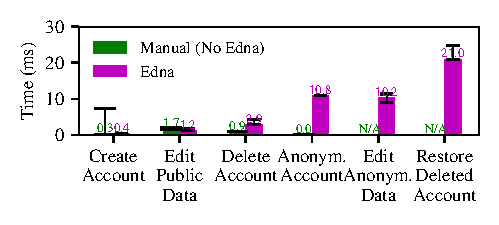
\includegraphics{figs/websubmit_op_stats}
    \caption{WebSubmit (2k users, 80 answers/user).}
    \label{f:ops-websubmit}
  \end{subfigure}
  \begin{subfigure}[b]{\columnwidth}
    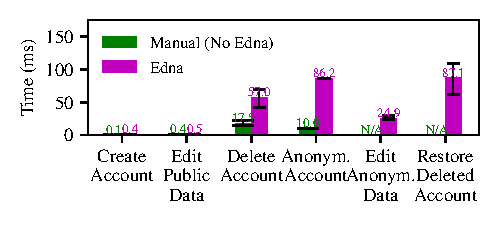
\includegraphics{figs/hotcrp_op_stats}
      \caption{HotCRP (80 reviewers, 3k total users, 155 records/reviewer).}
    \label{f:ops-hotcrp}
  \end{subfigure}
  \begin{subfigure}[b]{\columnwidth}
    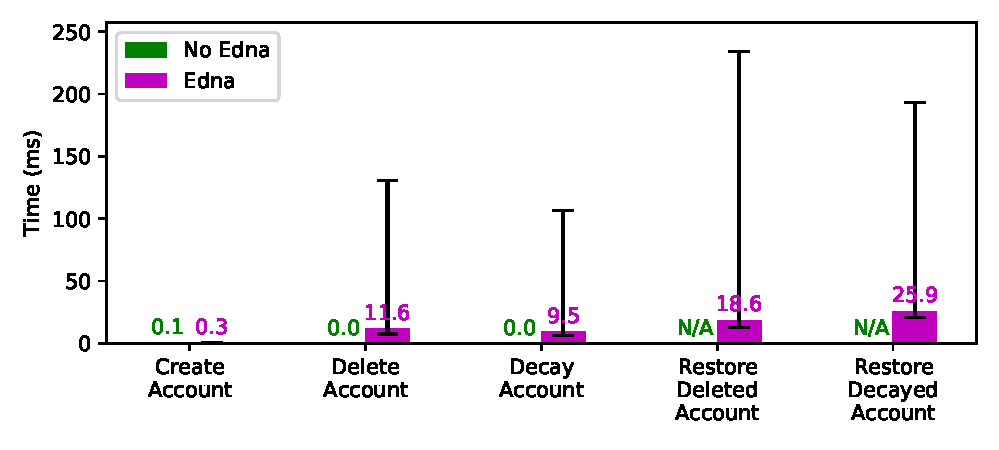
\includegraphics{figs/lobsters_op_stats}
    \caption{Lobsters (17.4k users, Zipf-distributed data/user).}
    \label{f:ops-lobsters}
  \end{subfigure}
  \caption{Latencies of disguise-related actions when implemented manually by the
  application developer without \sys, and with \sys.
  Each bar shows the median latency; ranges indicate the 5th to 95th
  percentile latencies.}
  \label{fig:client_opstats}
\end{figure}

\begin{figure}[t]
\centering
%\begin{tabular}{ c c }
%\textbf{DB Op} & \textbf{Time (ms)}\\
%\hline
%Update DB Row & 0.1\\
%Select DB Rows & 0.2\\
%Remove DB Rows & 0.2\\
%Reveal Deleted Row (DB Select + Insert) & 0.2 \\
%Create + Register Principal & 0.1\\
%\end{tabular}
%\quad
\begin{tabular}{ c c c c }
    \textbf{Crypto Op} & \multicolumn{3}{c}{\textbf{Time (ms)}}\\
\hline
    Generate Keypair & \multicolumn{3}{c}{301}\\
\hline
    & \textbf{Base (100B)} & \textbf{1MB} & \textbf{10MB}\\
    Encrypt Bag & 0.3 & 4.1 & 38.3\\
    Decrypt Bag & 2.8 & 4.5 & 22.3\\
\end{tabular}
  \caption{\sys cryptographic operations are cheap (0.3--4.5ms), except for
    pseudoprincipal key generation, which \sys amortizes by via a pre-generated
    key pool (\S\ref{s:impl}).}
  \label{f:opstats}
\end{figure}

\paragraph{WebSubmit.}
%
We run WebSubmit benchmarks with a database seeded with 2,000 users, 20
lectures with four questions each, and an answer for each question for
each user (160k total answers).
%
This might correspond to all classes in a department, or to a large AI class.
%
We measure end-to-end latency, which includes request processing in WebSubmit,
\sys's operations, and the response to the client.
%
The amount of data under disguise is constant across users, so we would expect
low variance in the results.
%

%
Figure~\ref{f:ops-websubmit} shows the median latency for two normal operations
(creating an account and editing unanonymized data), two disguises (delete account
and anonymizing an account), and two operations over data under disguise (editing
anonymized data and restoring the account).
%
Normal operations have comparable latencies with and without \sys.
%
\sys's disguise-based account deletion and anonymization take longer than the
baseline since \sys encrypts database diffs and speaks-for records, while
the baseline only deletes data from the application DB.
%
The absolute latency of \sys's disguises is 10.8ms and the latencies for
\sys's operations over data under disguise are 10--21ms.
%
(These operations are impossible in the baseline.)
%
However, WebSubmit's disguises are simple and touch at maximum two database
tables, so we repeate the same measurement with HotCRP's more complex schema and
disguises.
%

\paragraph{HotCRP.}
%
We run the HotCRP experiments on a database seeded with 450 total users (50 of
whom are PC members), 450 papers, and four reviews and four comments per paper,
distributed evenly among PC members.
%
The benchmark measures the server-side latency only.
%
HotCRP supports the same disguise-related operations as WebSubmit, but reviewers
have more data, and HotCRP's disguises mix deletions and decorrelations across
12 tables, so we would expect higher latencies.
%

%
Figure~\ref{f:ops-hotcrp} shows higher latencies in general, even for the manual
privacy transformations in the baseline, which reflects the more complex
disguises.
%
\sys takes 32--107ms to disguise and reveal a user's data, again owing to the
extra cryptographic operations necessary.
%
Note that account anonymization in HotCRP is an admin-applied disguises that
runs for all PC members.
%
Its total latency is proportional to the PC size; \eg with 50 PC members, it takes
five seconds, which is acceptable for a one-off operation.
%
As before, \sys adds minimal latency to normal application operations.
%

\paragraph{Lobsters.}
%
Finally, we consider Lobsters, which has users with far more variable amounts of
data.
%
We run Lobsters benchmarks on a database seeded with 17.4k users, 1.2x the
late-2021 size of the real Lobsters site~\cite{lobsters}.
%
These users have 120k stories, and 300k comments comments with votes;
stories, comments, and votes are distributed among users according to
statistics from the actual Lobsters deployment~\cite{lobsters-data}.
%
The benchmark measures server-side latency only, and we measure the account
decay disguise (and subsequent restoration) in addition to GDPR-compliant
account deletion and restoration.
%
Lobsters does not support editing decayed contributions.
%
As the amount of data per user follows a Zipf-like distribution, so we would
expect some users' disguises to be much more expensive than the median user's.
%

%
The results are in Figure~\ref{f:ops-lobsters}.
%
The median latencies are small (10--25ms for \sys, and <0.1ms for the
baseline), since the median Lobsters user has little data.
%
But some highly active users have a lot of data, which raises the
95\textsuperscript{th} percentile latency to 120--220ms for these users.
%

\paragraph{Summary.}
%
These results illustrate that data disguises are fast enough in absolute terms
that most of them could be run interactively as part of a web request.
%
Some global disguises---such as HotCRP's conference anonymization over many
users---take several seconds if run ad-hoc, but an application can also apply
these disguises incrementally by user in the background (as Lobsters's data decay
does).
%

%
\sys necessarily adds some latency compared to a manual privacy transformation
as it must encrypt and store data, as well as maintain its metadata.
%
Next, we break this down.
%

\subsubsection{\sys Per-Operation Drill-Down}
%
\sys's API calls perform three classes of primitive operations: data encryption
and decryption, store/retrieve accesses into \sys's store of encrypted bags,
and metadata updates.
%
\sys's high-level API additionally also operates on the application database,
while the application performs these queries when it uses \sys's low-level API.
%
\sys's store and metadata operations are fast; in our prototype, all of them
take less than 0.1ms.
%
The cost of application database operations depends on the amount of data
touched, but is in the single-digit milliseconds in our case studies.
%
\sys cryptographic operations are most expensive, and Figure~\ref{f:opstats}
shows their cost.
%

%
When disguises create pseudoprincipals, these pseudoprincipals need their
own keypair in case their data later gets disguised again.
%
Key generation is expensive ($\approx$300ms), and disguises would be
prohibitively slow if \sys incurred this latency for every pseudoprincipal
created.
%
To avoid this cost, \sys keeps a pre-generated key pool that it draws on
during disguises (\S\ref{s:impl}).
%
%
The baseline cost of encryption is 0.3ms, and grows linearly with data
size; baseline decryption cost is 2.8ms and also scales linearly.
%
A disguise or reveal operation requires a single encryption/decryption in
the simple case when the application only applied one disguise to the
data.
%
Several may be required when the application has applied multiple
disguises; we evaluate this cost next.
%

\begin{figure}[t]
    \centering
    \begin{subfigure}[b]{\columnwidth}
        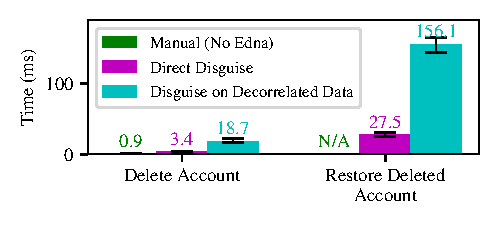
\includegraphics{figs/composition_stats_websubmit}
        \caption{WebSubmit}
        \label{f:comp-websubmit}
      \end{subfigure}
      \begin{subfigure}[b]{\columnwidth}
        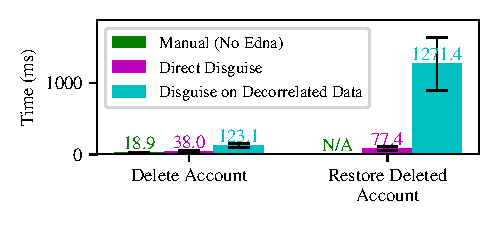
\includegraphics{figs/composition_stats_hotcrp}
          \caption{HotCRP}
        \label{f:comp-hotcrp}
      \end{subfigure}
    \caption{Disguise composition over a decorrelating account
      anonymization disguise increases latency proportionally
      to the amount of data touched, as \sys performs
      %3--5.5$\times$ and restoration by 5.7--10$\times$ as \sys
      crypto operations linear in the number of pseudoprincipals
      involved.}
    \label{f:composition}
\end{figure}

\subsubsection{Applying Multiple Disguises}
%
Our next experiment considers the cost of user-initiated account
deletion from an application that already invoked a prior disguise
to anonymize and decorrelate all users' data.
%
We consider WebSubmit and HotCRP, and compare three setups: \one{}
manual account deletion (as before); \two{} account deletion and
restoration \emph{without} prior a anonymization disguise; and
\three{} account deletion and restoration \emph{with} a prior
anonymization disguise.
%
When a natural principal deletes their account without a prior
disguise, \sys creates a single bag with all user data and encrypts
it as a batch.
%
But if the application applies the account deletion disguise over
data already decorrelated by anonymization, \sys associates any new
database diffs and speaks-for records with pseudoprincipals created
by anonymization.\footnote{Since this is an interactive disguise, \sys
can decrypt the natural principal's bag to find out which
pseudoprincipals' data to disguise. Without this bag access, \sys
by design can't know what data belongs to the deleted user.}
%
This requires \sys to create and encrypt
$O(\textit{\# pseudoprincipals})$ bags, so the disguise is necessarily
more expensive.
%
Account restoration follows a similar pattern: \sys takes the natural
principal's private key and locator, decrypts their bag, decrypts
the locator sets of the pseudoprincipals in that bag,
followed by decrypting the bags they point to (a linear number of
decryptions).
%
A good result for \sys would show a moderate increase in runtime,
proportional to the amount of user data already under disguise.
%

%%
%One such case occurs when a client interactively invokes $d_2$ on behalf of principal $p$ with private key $p$ and
%locators \lcapa{pd_1} from anonymization disguise $d_1$, the application can ask \sys (via
%\fn{PseudoprincipalsOf}) to decrypt all speaks-for records in $p$'s bag at \lcapa{pd_1} using $p$'s
%private key.
%This adds the cost of decrypting speaks-for records stored at \lcapa{pd_1}.
%%
%With these speaks-for tokens, the application and \sys can not only disguise
%$p$'s data, but also disguise data of $p$'s pseudoprincipals $q_i$ produced by $d_1$.
%\sys must perform one bag encryption \emph{per pseudoprincipal $q_i$}, rather than a single
%encryption for single pseudoprincipal $p$ had $p$'s data never been decorrelated by $d_1$.
%%
%
%%
%As described in \S\ref{s:composition}, the application and \sys return a locator \lcapa{pd_2} to the
%client for every $q_i$ disguised, which points to $q_i$'s encrypted bag of records.
%%
%Upon reveal of $d_2$ with $p$'s private key and locators from $d_1$ and $d_2$, \sys decrypts and
%reveals all bags for both $p$ and the $q_i$. Similarly, \sys must perform one decryption per $q_i$; without
%composition, \sys could simply perform a single decryption of $p$'s bag at \lcapa{pd_1}.

Figure~\ref{f:composition} shows the disguise latencies.
%
WebSubmit account deletion latency increases by 5.5$\times$ and restoration by 5.7$\times$; in
HotCRP, deletion latency increases by 3$\times$ and restoration latency by 10$\times$.
%
Accounts in HotCRP have more data, and 7--8$\times$ more pseudoprincipals per user after
anonymization than accounts in WebSubmit, so greater slowdowns in HotCRP make sense.
%
Restoring an account (\ie undoing a composed disguise) is more expensive than deleting an
account (\ie composing a disguise atop another) because decryption is more expensive than
encryption (Figure~\ref{f:opstats}).
%
Importantly, however, the disguise latencies are stable when \sys composes further
disguises atop these two: the cost is proportional to the number of pseudoprincipals
affected, and once the application has maximally decorrelated data (\ie one pseudoprincipal
per record), this number is stable.
%

%
The experiment composed an interactive disguise (account delete) atop a
non-interactive one (anonymization).
%
Interactive disguises let natural principals introduce locators for
pseudoprincipal-owned bags that \sys forgot, which helps avoid the locator
decryption step on revealing the composed disguise.
%
Composing a non-iteractive disguise requires this step as \sys stores the
locators, but avoids the one-off cost of decrypting a natural
principal's bag; overall, the cost is still linear in the number of
pseudoprincipals touched.
%

%%%%%%%%%%%%%%%%%%%%%%%%%%%%%%%%%%%%%%%%%%%%%%%%%%%%%%%%%%%%%%%%%%%%%%%%
\subsection{Space Used By \sys}
\label{s:eval-res}

%
Each generated pseudoprincipal adds an additional users object to the application
database.
%
\sys also stores public-key metadata for each active principal and
pseudoprincipal, metadata about which pseudopricipals to be forgotten,
encrypted ciphertexts for records, and an in-memory pool of pregenerated
private-public keypairs.
%
Clients keep track of keys and locators, but these are small and encoded
in application-specific ways.
%
To understand \sys's space footprint, we measure the size of all data stored
by \sys before and after 1.7k random users in Lobsters (10\% of users)
deleted their accounts.
%
Cryptographic material necessarily adds some overhead, and most of \sys's
state can be on persistent storage.
%

%
Prior to any account deletion, \sys's metadata (public keys of natural
principals) and the in-memory pool of keypairs uses 4.3 MB.
%
After the users delete their accounts, \sys's stores 137 MB of data.
%
The space used is primarily proportional to the number of pseudoprincipals
produced: each pseudoprincipal requires storing 1.4 KB of speaks-for
record, dominated by the private key (1.1 KB).
%
Deleting 10\% of Lobsters users produces 78.7k pseudoprincipals that use
110 MB.
%
Storing a private key is necessary if the application wants to further
disguise decorrelated data, but avoidable if disguises cannot compose.
%
In addition, each pseudoprincipal inserts a public key into \sys's
metadata, adding $\approx$0.3 KB per pseudoprincipal and 24 MB combined,
and \sys removes the public keys for the 1700 deleted natural principals.
%

%
The remaining $\approx$2.2 MB come from diff records that store the
user's deleted data from the application database; 2.2MB are 0.8\% of the
original Lobsters database size of 261 MB.

%%%%%%%%%%%%%%%%%%%%%%%%%%%%%%%%%%%%%%%%%%%%%%%%%%%%%%%%%%%%%%%%%%%%%%%%
\subsection{Impact On Concurrent Application Use}
\label{s:eval-conc}

%
Web applications serve many concurrent users, most of whom are simply using the
application.
%
Occasionally, a user (or an admin, or a cron job) will initiate a privacy
transformation, which invokes \sys.
%
These transformations are comparatively rare, but data disguises and \sys can
only be practical if the latency of normal application requests is largely
unaffected by \sys' disguise and reveal operations.
%
If an expensive disguise---such as a popular Lobsters user deleting their
account---blocked application processing for all other users, developers would
be rightly sceptical to deploy \sys.
%

\begin{figure}[t]
    \centering
%    \begin{subfigure}[b]{0.49\textwidth}
        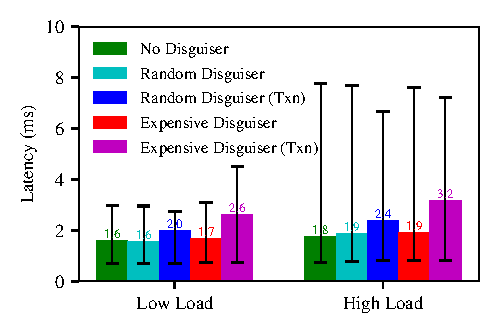
\includegraphics{figs/lobsters_concurrent_results}
        \caption{Even continuous disguise/reveal operations by a heavy-hitter user in Lobsters (>6k
          data objects) have a small impact on application request latency. Bars show median latency,
          error bars are the 5\textsuperscript{th}/95\textsuperscript{th} percentiles.}
        \label{f:concurrent-lobsters}
%    \end{subfigure}
%    \begin{subfigure}[b]{0.49\textwidth}
%        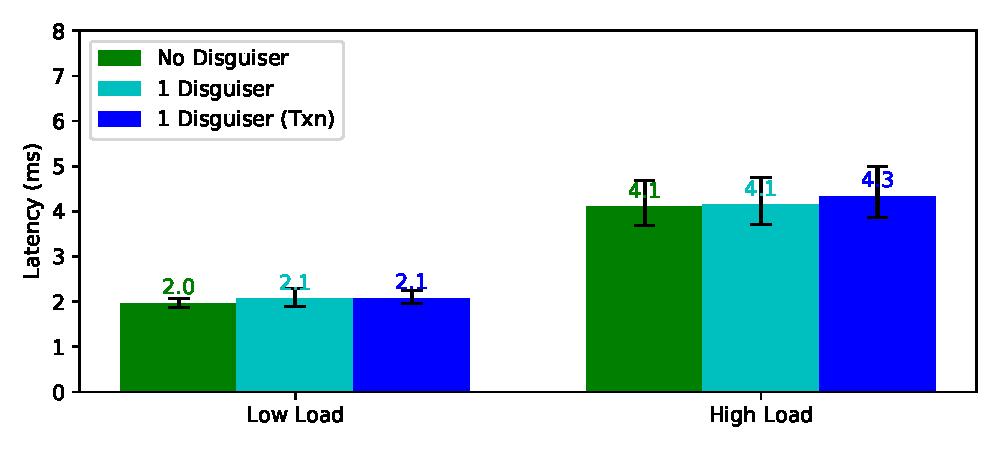
\includegraphics{figs/websubmit_concurrent_results}
%        \caption{WebSubmit. A user's continuous disguising/revealing has only a small impact on
%          application request latency.}
%        \label{f:concurrent-websubmit}
%    \end{subfigure}
%    \caption{Impact of continuously applying and revealing account deletion disguises (with and with TX
%    over the application DB) on other users' concurrent application requests. Bars show median latency,
%    error bars indicate 5\textsuperscript{th}/95\textsuperscript{th} percentiles.}
%    \label{fig:concurrent}
\end{figure}

%
We investigate the impact of \sys's disguise and reveal operations, as well as
operations over data under disguise, on other concurrent user requests in Lobsters.
%
In both experiments, a set of ``normal'' users make requests to the application
while another (distinct) set of users continuously deletes and restores their
accounts.
%
\sys applies disguises sequentially, so only one disguise happens at a time.
%
(This is realistic, as the UI can tell other users to wait or process the request
asynchronously; it also avoids \sys having to reason about overlapping data between
two or more disguises.)
%
We measure the latency of ``normal'' user's application operations in closed-loop
setting, both without any disguises (the baseline) and with the application
continuously invoking \sys.
%
Our Lobsters application workload is based on the request distributions in the real
Lobsters deployment~\cite{lobsters-data}.
%
Since the disguise/reveal cost in Lobsters varies across users, we measure the
impact of randomly chosen users invoking account deletion/restoration, and of
the user with the most data continuously deleting and restoring their account
(a worst-case scenario for this application).
%
We show latency in a low load scenario ($\approx$10\% CPU load on the server),
and a high load scenario in which we run the maximum load supported before
concurrency control in the MariaDB database becomes a bottleneck
and throughput increases no further (at $\approx$40\% CPU load).
%
Finally, we measure a setting without using a transaction for the disguise's
application database operations, and one with such a transaction.
%
The latter makes sense sense if the application wishes to avoid exposing
partially-disguised data to other clients.
%
A good result for \sys would show little impact on the latency of normal operations
when concurrent privacy transformations occur.
%

%
Figure~\ref{f:concurrent-lobsters} shows the results.
%
The median latency of normal application requests increases by 6--38\% (from
1.6ms to 1.7ms under low load, and 1.8ms to 1.9--2.5ms under high load) when
random users delete and restore their accounts.
%
Transactional account deletion and restoration of the most expensive user
results in a 11--38\% increase in median latency.
%
These results show that \sys's data disguises, as well as operations over data under disguise (here,
account restoration) have little impact on other user's application experience.
%

%
While the experiment measured normal application request latency, the
account deletions and restorations performed with high load take 9ms and
15ms to complete in the median.
%
The expensive user's account deletion and reveal take 2--3 seconds.
%
We believe this is acceptable, as disguises aren't time-critical.
%
